\documentclass[oneside,authoryear,spanish]{ezthesis}
\usepackage{float}
\usepackage{natbib}

%% # Opciones disponibles para el documento #
%%
%% Las opciones con un (*) son las opciones predeterminadas.
%%
%% Modo de compilar:
%%   draft            - borrador con marcas de fecha y sin im'agenes
%%   draftmarks       - borrador con marcas de fecha y con im'agenes
%%   final (*)        - version final de la tesis
%%
%% Tama'no de papel:
%%   letterpaper (*)  - tama'no carta (Am'erica)
%%   a4paper          - tama'no A4    (Europa)
%%
%% Formato de impresi'on:
%%   oneside          - hojas impresas por un solo lado
%%   twoside (*)      - hijas impresas por ambos lados
%%
%% Tama'no de letra:
%%   10pt, 11pt, o 12pt (*)
%%
%% Espaciado entre renglones:
%%   singlespace      - espacio sencillo
%%   onehalfspace (*) - espacio de 1.5
%%   doublespace      - a doble espacio
%%
%% Formato de las referencias bibliogr'aficas:
%%   numbers          - numeradas, p.e. [1]
%%   authoryear (*)   - por autor y a'no, p.e. (Newton, 1997)
%%
%% Opciones adicionales:
%%   spanish         - tesis escrita en espa'nol
%%
%% Desactivar opciones especiales:
%%   nobibtoc   - no incluir la bibiolgraf'ia en el 'Indice general
%%   nofancyhdr - no incluir "fancyhdr" para producir los encabezados
%%   nocolors   - no incluir "xcolor" para producir ligas con colores
%%   nographicx - no incluir "graphicx" para insertar gr'aficos
%%   nonatbib   - no incluir "natbib" para administrar la bibliograf'ia

%% Paquetes adicionales requeridos se pueden agregar tambi'en aqu'i.
%% Por ejemplo:
%%\usepackage{subfig}
%\usepackage{multirow}
%%\usepackage{fontspec}
\usepackage{soul}
\usepackage{enumerate}
\usepackage{natbib}
\usepackage{longtable, booktabs}
\usepackage{dcolumn}
\usepackage{listings}
\usepackage{xcolor}

\definecolor{codegreen}{rgb}{0,0.6,0}
\definecolor{codegray}{rgb}{0.5,0.5,0.5}
\definecolor{codepurple}{rgb}{0.58,0,0.82}
\definecolor{backcolour}{rgb}{0.95,0.95,0.92}

\lstdefinestyle{mystyle}{
    backgroundcolor=\color{backcolour},   
    commentstyle=\color{codegreen},
    keywordstyle=\color{magenta},
    numberstyle=\tiny\color{codegray},
    stringstyle=\color{codepurple},
    basicstyle=\ttfamily\footnotesize,
    breakatwhitespace=false,         
    breaklines=true,                 
    captionpos=b,                    
    keepspaces=true,                 
    numbers=left,                    
    numbersep=5pt,                  
    showspaces=false,                
    showstringspaces=false,
    showtabs=false,                  
    tabsize=2
}

\lstset{style=mystyle}
\setlength{\headheight}{15.71667pt}
\addtolength{\topmargin}{-0.71667pt}

%% # Datos del documento #
%% Nota que los acentos se deben escribir: \'a, \'e, \'i, etc.
%% La letra n con tilde es: \~n.

\author{Dimitrio Mandamadiotis Kalfagiannis}
\title{Desarrollo de un sistema para inferir la deserci\'on de los clientes en un e-commerce}
\degree{Ingeniero de Sistemas}
\supervisor{\\ Yaneth Moreno, M.Sc}
\institution{Universidad de Los Andes}
\faculty{Facultad de Ingenier\'ia}
\department{Escuela de Sistemas}
\department{Departamento de Sistemas Computacionales}

%% # M'argenes del documento #`
%% 
%% Quitar el comentario en la siguiente linea para austar los m'argenes del
%% documento. Leer la documentaci'on de "geometry" para m'as informaci'on.

%\geometry{top=40mm,bottom=33mm,inner=40mm,outer=25mm}

%% El siguiente comando agrega ligas activas en el documento para las
%% referencias cruzadas y citas bibliogr'aficas. Tiene que ser *la 'ultima*
%% instrucci'on antes de \begin{document}.
\hyperlinking
\begin{document}

%% En esta secci'on se describe la estructura del documento de la tesis.
%% Consulta los reglamentos de tu universidad para determinar el orden
%% y la cantidad de secciones que debes de incluir.

%% # Portada de la tesis #
%% Mirar el archivo "titlepage.tex" para los detalles.
%% ## Construye tu propia portada ##
%% 
%% Una portada se conforma por una secuencia de "Blocks" que incluyen
%% piezas individuales de informaci'on. Un "Block" puede incluir, por
%% ejemplo, el t'itulo del documento, una im'agen (logotipo de la universidad),
%% el nombre del autor, nombre del supervisor, u cualquier otra pieza de
%% informaci'on.
%%
%% Cada "Block" aparece centrado horizontalmente en la p'agina y,
%% verticalmente, todos los "Blocks" se distruyen de manera uniforme 
%% a lo largo de p'agina.
%%
%% Nota tambi'en que, dentro de un mismo "Block" se pueden cortar
%% lineas usando el comando \\
%%
%% El tama'no del texto dentro de un "Block" se puede modificar usando uno de
%% los comandos:
%%   \small      \LARGE
%%   \large      \huge
%%   \Large      \Huge
%%
%% Y el tipo de letra se puede modificar usando:
%%   \bfseries - negritas
%%   \itshape  - it'alicas
%%   \scshape  - small caps
%%   \slshape  - slanted
%%   \sffamily - sans serif
%%
%% Para producir plantillas generales, la informaci'on que ha sido inclu'ida
%% en el archivo principal "tesis.tex" se puede accesar aqu'i usando:
%%   \insertauthor
%%   \inserttitle
%%   \insertsupervisor
%%   \insertinstitution
%%   \insertdegree
%%   \insertfaculty
%%   \insertdepartment
%%   \insertsubmitdate
%%\begin{figure}[h]
%%\centering
\begin{center}
\TitleBlock[\bigskip]{}

\includegraphics[width=0.15\textwidth]{images/logoULA.jpg}
\\[5mm]PROYECTO DE GRADO
\\[1cm]Presentado ante la ilustre Universidad de Los Andes como requisito final para obtener el T'itulo de Ingeniero de Sistemas
\end{center}
%%\caption{ }
%%\end{figure}
 

\begin{titlepage}
 %% \TitleBlock{\scshape\insertinstitution}
  %%\TitleBlock[\bigskip]{\scshape\insertfaculty}
   %%\TitleBlock[\bigskip]{\scshape\insertdepartment}
   %%\TitleBlock[\bigskip]{\scshape }
   
  %% \TitleBlock{\normalsize\scshape\inserttitle}
  %% \TitleBlock{\scshape
 %Presentado ante la ilustre \insertinstitution\ como requisito final\\ %%\insertauthor \\
%  para obtener el T'itulo de \insertdegree \\
  \vspace*{0.50in}
  
 	\TitleBlock{\normalsize\scshape\inserttitle}
  \TitleBlock{\scshape
  	Br. \insertauthor\\

    Tutores: \insertsupervisor\\
    }
  \TitleBlock{\scshape
    M'erida, Febrero de \insertsubmitdate}
\end{titlepage}

%% Nota 1:
%% Se puede agregar un escudo o logotipo en un "Block" como:
%%   \TitleBlock{\includegraphics[height=4cm]{escudo_uni}}
%% y teniendo un archivo "escudo_uni.pdf", "escudo_uni.png" o "escudo_uni.jpg"
%% en alg'un lugar donde LaTeX lo pueda encontrar.

%% Nota 2:
%% Normalmente, el espacio entre "Blocks" se extiende de modo que el
%% contenido se reparte uniformemente sobre toda la p'agina. Este
%% comportamiento se puede modificar para mantener fijo, por ejemplo, el
%% espacio entre un par de "Blocks". Escribiendo:
%%   \TitleBlock{Bloque 1}
%%   \TitleBlock[\bigskip]{Bloque2}
%% se deja un espacio "grande" y de tama~no fijo entre el bloque 1 y 2.
%% Adem'as de \bigskip est'an tambi'en \smallskip y \medskip. Si necesitas
%% aun m'as control puedes usar tambi'en, por ejemplo, \vspace*{2cm}.




%% # Prefacios #
%% Por cada prefacio (p.e. agradecimientos, resumen, etc.) crear
%% un nuevo archivo e incluirlo aqu'i.
%% Para m'as detalles y un ejemplo mirar el archivo "gracias.tex".
%%% Las secciones del "prefacio" inician con el comando \prefacesection{T'itulo}
%% Este tipo de secciones *no* van numeradas, pero s'i aparecen en el 'indice.
%%
%% Si quieres agregar una secci'on que no vaya n'umerada y que *tampoco*
%% aparesca en el 'indice, usa entonces el comando \chapter*{T'itulo}
%%
%% Recuerda que aqu'i ya puedes escribir acentos como: 'a, 'e, 'i, etc.
%% La letra n con tilde es: 'n.

\prefacesection{Agradecimientos}

Este trabajo no habr'ia sido posible sin el apoyo y el est'imulo de mi colega
y amigo, Doctor Rudolf Fliesning,  bajo cuya supervisi'on escog'i este tema y
comenc'e la tesis. Sr. Quentin Travers, mi consejero en las etapas finales
del trabajo, tambi'en ha sido generosamente servicial, y me ha ayudado de
numerosos modos, incluyendo el resumen del contenido de los documentos que
no estaban disponibles para mi examen, y en particular por permitirme leer, 
en cuanto estuvieron  disponibles, las copias de los  recientes extractos de
los diarios de campa'na del Vigilante Rupert Giles y la actual Cazadora la
se'norita Buffy Summers, que se encontraron con William the Bloody en 1998, y
por facilitarme el pleno acceso  a los diarios de anteriores Vigilantes
relevantes a la carrera de William the Bloody.

Tambi'en me gustar'ia agradecerle al Consejo la concesi'on de Wyndham-Pryce
como Compa'nero, el cual me ha apoyado durante mis dos a'nos de investigaci'on,
y la concesi'on de dos subvenciones de viajes, una para estudiar documentos
en los Archivos de Vigilantes sellados en Munich, y otra para la
investigaci'on en campa'na en Praga. Me gustar'ia agradecer a Sr. Travers,
otra vez, por facilitarme  la acreditaci'on  de seguridad para el trabajo en
los Archivos de Munich, y al Doctor Fliesning por su apoyo colegial y ayuda
en ambos viajes de investigaci'on.

No puedo terminar sin agradecer a mi familia, en cuyo est'imulo constante y
amor he confiado a lo largo de mis a'nos en la Academia. Estoy agradecida
tambi'en a los ejemplos de mis  difuntos hermano, Desmond Chalmers, Vigilante
en Entrenamiento, y padre, Albert Chalmers, Vigilante. Su coraje resuelto
y convicci'on siempre me inspirar'an, y espero seguir, a mi propio y peque'no
modo, la noble misi'on por la que dieron sus vidas. Es a ellos a quien dedico
este trabajo.

%% Por si alguien tiene curiosidad, este "simp'atico" agradecimiento est'a
%% tomado de la "Tesis de Lydia Chalmers" basada en el universo del programa
%% de televisi'on Buffy, la Cazadora de Vampiros.
%% http://www.buffy-cazavampiros.com/Spiketesis/tesis.inicio.htm


%% # 'Indices y listas de contenido #
%% Quitar los comentarios en las lineas siguientes para obtener listas de
%% figuras y cuadros/tablas.
\tableofcontents
%\listoffigures
%\listoftables

%% # Cap'itulos #
%% Por cada cap'itulo hay que crear un nuevo archivo e incluirlo aqu'i.
%% Mirar el archivo "intro.tex" para un ejemplo y recomendaciones para
%% escribir.
%% Los capitulos inician con \chapter{T'itulo}, estos aparecen numerados y
%% se incluyen en el 'indice general.
%%
%% Recuerda que aqu'i ya puedes escribir acentos como: 'a, 'e, 'i, etc.
%% La letra n con tilde es: 'n.

\chapter{Introducci'on}

El comercio electrónico o también conocido como e-commerce, consiste en la compra y venta de productos o servicios a través de internet, este comenzó a principios de 1970 y se desarrolló a mediados de la década de los 90 como una manera bastante sencilla de adquirir productos o servicios sin tener que desplazarse a una ubicación física.


La cantidad de comercio llevada a cabo electrónicamente ha crecido de manera extraordinaria y esto ha estimulado la creación y utilización de innovaciones como el marketing en internet, cadenas de suministros complejas, sistemas automáticos de recolección de datos y sistemas para la gestión de la relación con el cliente, estos últimos han permitido la aplicación de métodos cuantitativos para el análisis y la optimización del rendimiento en los e-commerce.


Una de las áreas más importantes de estudio es el comportamiento de los clientes, en ella se evalúa y se estudia la relación directa que existe entre el servicio que se les proporciona a los usuarios y los ingresos de la tienda de comercio electrónico, para esto se utilizan variables como el valor del ciclo de vida de un cliente y la tasa de churn y lo que se busca es obtener un incremento en las ventas mediante mejoras en los servicios, la experiencia del cliente y la calidad de los productos.

\section{Antecedentes}

En el mundo de los negocios y el comercio actual seguimos observando un crecimiento rápido de los sistemas digitales y las tecnologías de información, algunos de estos sistemas se basan en la gestión de relaciones con los clientes, los cuales son comunes en negocios contractuales como los servicios de telecomunicaciones o servicios de software basado en suscripción. El comercio electrónico es un negocio no contractual y en Europa tiene un crecimiento anual proyectado del 6 \% hasta el año 2025, también en el año 2020 los ingresos en e-commerce aumentaron en un 10 \% (Jílková \& Králová, 2021) \cite{Jilkova2021}, estas cifras nos demuestran lo vital que es para los negocios mantener a los clientes.


Durante los últimos tres años se han realizado muchos estudios sobre el comportamiento de los clientes en los negocios. (Falla, 2021) \cite{Falla2022} en su trabajo de grado Predicción de Abandono de Clientes en Telecomunicaciones Mediante el Aprendizaje Automático, utiliza técnicas y algoritmos de inteligencia artificial para predecir el abandono de clientes en un negocio con modelo contractual. También identificó varias técnicas de minería de datos para la identificación de clientes que están a punto de abandonar.


(Sinha \& Raizada,  2022) \cite{SinhaRaizada2022} en su trabajo Modelling Customer Churn Rate and Its Use for Customer Retention Planning muestran un modelo para un negocio contractual basado en máquinas de aprendizaje o machine learning para predecir la tasa de abandono, adicionalmente dan una serie de recomendaciones a los negocios para mantener una tasa de abandono baja según sus descubrimientos.


La complejidad de modelar la tasa de abandono en negocios no contractuales viene de que no se conoce el momento en el que un cliente abandonó. Una manera de aproximar esta variable es mediante el valor de la compra media de un cliente. (Abdolvand, Albadvi \& Koosha, 2021) \cite{AbdolvandAlbadviKoosha2021} mencionan en su artículo Customer Lifetime Value: Literature scoping map, and an agenda for future research que la literatura se enfoca en explicaciones teóricas para calcular el valor de la compra media de un cliente, pero no expresan las diferencias que pueden existir a la hora de aplicar el conocimiento a la práctica.


\section{Planteamiento del problema}

En un negocio como una tienda de comercio electrónico lo más importa son los clientes, sin ellos no hay ingresos y sin ingresos la tienda no podría existir. En la actualidad el costo de atraer y convertir personas en nuevos clientes suele ser muy alto, además, es mucho más fácil vender productos a un individuo que ya ha comprado antes en la tienda que a un desconocido, es por esto que vale la pena determinar cuándo los clientes podrían desertar para poder tomar acción antes y tratar de prevenir el abandono. Por otro lado, es esencial determinar con precisión cuántos de los clientes aún siguen siéndolo, con esta información se podría analizar el estado actual del negocio y proyectar escenarios para el futuro.


Calcular el churn de los clientes es más fácil en negocios contractuales, como proveedores de telefonía o de banda ancha, ya que es fácil determinar cuándo estos están a punto de abandonar a medida que sus contratos se acercan a la fecha de finalización. Sin embargo, predecir la deserción en mercados no contractuales como el comercio electrónico es mucho más difícil porque no se conoce el momento de salida de un cliente, y en su lugar debe predecirse.


En este sentido, se considera que desarrollar un sistema capaz de predecir el churn de los clientes en un e-commerce sería de vital importancia, ya que permitiría analizar la salud de un negocio y le daría una ventaja a los administradores y encargados de área de marketing.

\section{Justificación}

El comercio electrónico a nivel mundial ha tenido un crecimiento exponencial en los últimos años y debido a esto se ha generado una cantidad gigantesca de datos que se pueden utilizar para optimizar métricas y alcanzar objetivos de negocio.


En los negocios contractuales es fácil establecer una base para analizar el comportamiento de los usuarios, esto porque se conoce con exactitud la cantidad de usuarios que dejaron de ser clientes en un momento dado, ya que no renovaron sus contratos o suscripciones. Estos datos permiten a los negocios contractuales crear sistemas complejos de predicciones de rendimiento y la optimización de la experiencia del usuario.


Dicho esto, hay otro grupo de negocios donde no se sabe con exactitud cuando un usuario deja de ser cliente. Es por ello que es necesario definir un sistema para predecir la deserción de los clientes en los negocios no contractuales como las tiendas de comercio electrónico. Este sistema le da la posibilidad a estos negocios de realizar análisis complejos e identificar problemas en las relaciones con sus clientes y tomar acción para prevenir el abandono a tiempo.

\section{Objetivos}

El objetivo general de este trabajo de grado es desarrollar un sistema capaz de inferir la deserción de los clientes en una tienda de comercio electrónico.


Para ello se debe cumplir con los siguientes objetivos específicos:


\begin{enumerate}
	\item Construir un data Warehouse con información sobre patrones de comportamiento de los clientes en una tienda de comercio electrónico.
	\item Definir el método estadístico apropiado para inferir la deserción de los clientes.
	\item Desarrollar el modelo para inferir la deserción de los clientes en una tienda de comercio electrónico.
	\item Validar el modelo desarrollado con un conjunto de datos de prueba.
	\item Evaluar el rendimiento del modelo.
\end{enumerate}

\section{Metodología}


	En la actualidad, la agilidad al cambio es un factor de suma importancia en los proyectos que involucren software. Los requisitos y diseños tienden a cambiar rápidamente con el tiempo para adaptarse a las necesidades del proyecto. Por esta razón, existen las metodologías ágiles, estas permiten darle un mayor enfoque al proceso de desarrollo, enfatizar la comunicación cara a cara en lugar de la documentación y en especial facilitar la refactorización y la adaptación a los cambios. En este proyecto se plantea aplicar el método Kanban combinado con un backlog, esto facilita la organización y optimiza el flujo del trabajo para la investigación y el desarrollo del sistema. 


	Kanban se basa en una estructura de flujo de trabajo continuo de forma visual. Los elementos de trabajo que son representados por tarjetas se organizan en un tablero de kanban, donde pasan de una etapa del flujo de trabajo (columna) a la siguiente. Las etapas habituales del flujo de trabajo son:


\begin{itemize}
	\item \textbf{Por hacer:} que representa el trabajo que no se ha empezado.
	\item \textbf{En curso:} trabajo en el que se está trabajando activamente.
	\item \textbf{En revisión:} trabajo que está finalizado y en espera de revisión.
	\item \textbf{Finalizado:} trabajo completamente terminado.
\end{itemize}


	Una característica importante de kanban es que se establece una cantidad máxima de trabajo que puede existir en cada estado del flujo de trabajo. Limitar la cantidad de trabajo en curso mejora el rendimiento y reducen la cantidad de trabajo “prácticamente listo”, ya que obliga al equipo a centrarse en un conjunto de tareas más pequeño, en este proyecto no se podrá trabajar en más de tres tareas activas. Esta característica puede ser una limitante a la hora de programar las tareas por hacer, es por ello que se va a tratar esta columna como un backlog.


	El backlog es una lista de trabajo ordenado por prioridades para el equipo de desarrollo que se obtiene de la hoja de ruta y los requisitos. Los elementos más importantes se muestran al principio del backlog para que el equipo sepa qué hay que entregar primero. En este proyecto el backlog será atendido por el tutor y el autor.

\section{Alcances}

En el presente proyecto se plantea la creación de un sistema que analice los datos relacionados al comportamiento de los usuarios en un sitio web de comercio electrónico, específicamente el historial de transacciones de los usuarios en la tienda. Estos datos servirán de entrada a un modelo que tendrá como salida la probabilidad de que el usuario abandonara la tienda en un momento en el futuro.

El sistema tendrá una interfaz web donde un usuario podrá ingresar a través de un formulario el historial de transacciones de sus clientes, luego el sistema procesará la información y mostrará un gráfico por cada uno de los clientes, este gráfico mostrará la probabilidad de deserción del cliente desde su primera compra hasta 500 días en el futuro.

Para la programación del sistema se hará uso del lenguaje Python para la implementación del modelo ya que es el lenguaje mas utilizado en el área de análisis de datos y la mayoría de las herramientas están codificadas en este lenguaje. Para desarrollar la interfaz web se utilizará el lenguaje Javascript, el framework VueJS y el metaframework Nuxt para el frontend. Para el backend se usará Python y la biblioteca Flask.  
%% Los capitulos inician con \chapter{T'itulo}, estos aparecen numerados y
%% se incluyen en el 'indice general.
%%
%% Recuerda que aqu'i ya puedes escribir acentos como: 'a, 'e, 'i, etc.
%% La letra n con tilde es: 'n.

\chapter{Marco Referencial}

En éste capítulo, se pretende explicar las bases teóricas necesarias para la comprensión del diseño e implementación de un sistema para inferir la deserción de clientes en un e-commerce.

\section{E-Commerce}

Se puede definir al comercio electrónico o E-Commerce como transacciones comerciales realizadas digitalmente entre individuos y organizaciones. Las transacciones comerciales implican un intercambio de valor (por lo general dinero) o comercio entre las partes interesadas a cambio de productos o servicios. El hecho de que se realicen las transacciones digitalmente supone el uso de tecnologías digitales como la internet, la web, dispositivos electrónicos y software.

\subsubsection{Cliente}

Un cliente en el contexto del comercio electrónico es un individuo que realiza compras regulares a través de algún canal digital de una organización. El proceso de compra de este cliente es similar al de una tienda física y consiste en: visualizar los productos o servicios que ofrece la organización, luego procede a agregar lo que desea comprar a un carrito de compras, cuando el cliente está listo para pagar, el carrito es verificado y luego pagado de forma digital, finalmente se genera un registro de pedido en el sistema el cual es procesado por la organización para satisfacer la compra.

\subsubsection{Pedido}

Un pedido u orden de compra es un registro que contiene información relevante sobre una transacción de compra realizada por un cliente en una plataforma de comercio electrónico de una organización. Este registro suele contener información relevante a los procesos de cada organización pero los datos indispensables que incluye son: la fecha en que se realizó un pedido, el valor monetario del mismo y el cliente que lo generó.

\subsubsection{Negocio Contractual}

Se considera negocio contractual a toda organización que interactué y trabaje con sus clientes bajo el modelo de suscripción u otra configuración contractual. En este tipo de organizaciones es relativamente fácil determinar si un cliente está activo o no, ya que por lo general se registran los datos de vencimiento y renovación de contratos o suscripciones. Algunos ejemplos de negocios contractuales son las compañías de seguros, empresas de telecomunicaciones, gimnasios y plataformas SaaS.

\subsubsection{Negocio No Contractual}

Un negocio no contractual es cuando la organización no tiene mecanismo que le ayude a determinar cuando la relación con un individuo o cliente ha finalizado, esto debido a que un cliente puede estar en un periodo de espera antes de realizar otra compra o puede que no compre de nuevo a la organización. Ejemplos de este tipo de negocio son las tiendas de comercio electrónico y las tiendas de venta al por menor.

\subsubsection{Deserción de Clientes (Churn)}

Deserción de clientes o Churn es la pérdida de clientes debido al desgaste y es lo opuesto a la retención de clientes. Ésta se considera una métrica crucial para las empresas y se utiliza como base para calcular otras métricas de gran importancia como la vida útil del cliente, el valor de vida útil (CLV por sus siglas en inglés), el gasto de adquisición de clientes y el gasto de éxito del cliente.

\subsubsection{Valor de vida útil de un cliente (CLV)}

Esta medida representa el valor que tiene un cliente para un negocio a lo largo de toda la relación, es decir, es el valor total que ha aportado un cliente al negocio desde que realizó una primera compra, hasta que desertó.

\section{Modelo}

En líneas generales, un modelo es una representación de un sistema, éste se compone por conceptos que ayudan a explicar el sistema, estudiar los efectos de diferentes componentes y hacer predicciones sobre el comportamiento del mismo. Estos conceptos suelen manifestarse en un grupo de ecuaciones matemáticas.

\subsection{Modelo Estadístico}

Un modelo estadístico es un modelo matemático que representa una o varias suposiciones estadísticas, estas suposiciones tienen describen propiedades que nos permiten calcular la probabilidad de que ocurra un evento.

\subsection{Modelos Buy-Till-You-Die (BTYD)}

Son una familia de modelos estadísticos que tienen como objetivo describir el comportamiento de compra de los clientes como una serie de distribuciones. Estos modelos se basan en dos suposiciones básicas:

\begin{enumerate}
	\item Los clientes interactúan con la organización cuando están activos o "vivos".
	\item Los clientes pueden “morir” o transformarse en clientes inactivos después de un periodo de tiempo.
\end{enumerate}

Existen varios modelos BTYD, pero todos tienen las siguientes características:

\subsubsection{Modelado Probabilístico}

Todos estos modelos generan distribuciones de probabilidad para describir el comportamiento de los clientes. Si bien los modelos difieren en cómo crean estas distribuciones o cómo se ven estas distribuciones, todos comparten este objetivo principal.

\subsubsection{Tabla de pedidos}

La entrada requerida para generar las predicciones en todos los modelos BTYD es simplemente una tabla que contenga los pedidos de los clientes.  Cada modelo procesa esta tabla de manera diferente, pero todos comparten una estructura de entrada común. Debido a este requisito de entrada, cuantos más datos longitudinales se tenga sobre los pedidos de los clientes, más sólidas serán las predicciones del modelo.

\subsubsection{Análisis RFM}

 El modelado y análisis de RFM es una estrategia común empleada actualmente por las empresas para capturar el comportamiento del cliente y clasificarlo según tres variables: 
 
\begin{itemize}
	\item \textbf{Recencia (Recency):} ¿Hace cuánto tiempo compró un cliente? Este dato hace referencia a la duración en periodos de tiempo entre la primera compra del cliente y la última.	
	\item \textbf{Frecuencia (Frecuency):} ¿Con qué frecuencia/consistencia compra un cliente? Este valor representa la cantidad de periodos de tiempo en los que el cliente realizó un pedido.
	\item \textbf{Valor Monetario (Monetary):} ¿Cuánto gasta un cliente en promedio? Esto es la suma de todos los valores monetarios de las compras de un cliente dividida por el número total de compras.
\end{itemize}

Cada uno de estos elementos del análisis RFM juega un papel clave en las distribuciones del los modelos BTYD. 

\subsection{Modelo Pareto / NBD}

El nombre se refiere a la distribución de Pareto utilizada para modelar la deserción de clientes y la distribución binomial negativa (NBD) utilizada en la predicción de compras futuras. Este modelos asume que los clientes compran a un ritmo constante durante un periodo de tiempo y luego pasan a la inactividad.

	El objetivo del modelo Pareto / NBD es desarrollar el análisis RFM capturando el contexto del cliente al decidir si, el cliente ha desertado o no y con qué frecuencia comprará. Por ejemplo, si estudiamos un cliente A y un cliente B: 

\begin{itemize}
	\item El cliente A compró en una tienda de comercio electrónico cada dos días durante 2 meses. Sin embargo, no ha comprado en las últimas 2 semanas.
	\item El cliente B compró en la tienda aproximadamente una vez al mes durante los últimos 6 meses. Tampoco ha comprado en las últimas 2 semanas.
\end{itemize}

A pesar de que ambos clientes tienen la misma antigüedad (14 días), la diferencia en el comportamiento de compra cambia la probabilidad de deserción. Además, a pesar de comprar en la misma tienda, exhiben patrones de compra significativamente diferentes (cada dos días frente a cada mes), por lo que cualquier predicción debe tener en cuenta sus hábitos de compra.

El modelo de Pareto/NBD se basa en cinco supuestos:

Desde el punto de vista del cliente individual:

\begin{itemize}
	\item \textbf{Compras siguen la distribución Poisson:} Mientras está activo, el número de transacciones realizadas por un cliente en un período de tiempo de longitud t se representan mediante una distribución Poisson con media $\lambda t$. En realidad, Pareto/NBD, como su nombre lo indica, utiliza una distribución binomial negativa de la cual, la distribución de Poisson es un caso especial. La distribución de Poisson es una elección acertada para modelar el tiempo entre transacciones, ya que diferentes negocios tendrán diferentes tiempos y los clientes también pueden exhibir diferentes patrones de compra.
	\item \textbf{“Vida útil” exponencial:} Cada cliente tiene una "vida útil" no observada de longitud $\tau$. Este punto en el que el cliente se vuelve inactivo se distribuye exponencialmente con una tasa de deserción $\mu$. Esto lo que nos dice es que en general, la mayoría de los clientes se transformarán en inactivos relativamente rápido después de realizar una compra inicial pero una pequeña cohorte de clientes permanecerá durante mucho tiempo.
\end{itemize}

Heterogeneidad entre clientes:

\begin{itemize}
	\item \textbf{Las tasas de compra individuales siguen la distribución gamma:} la tasa de compra $\lambda$ para los diferentes clientes sigue una distribución gamma entre la población de clientes.
	\item \textbf{Tasa de deserción sigue distribuciones gamma diferentes:} Las tasas de deserción $\mu$ siguen una distribución gamma que es diferente entre los clientes.
	\item \textbf{Independencia de tasas:} Las tasas de transacciones $\lambda$ y las tasas de deserciones $\mu$ están distribuidas independientemente entre ellas.
\end{itemize}

Este modelo tiene mucho poder a la hora de analizar el comportamiento de clientes y requiere solo dos entradas sobre cada cliente, su "recencia" y "frecuencia". El modelo utiliza la inferencia de probabilidad logarítmica para hacer predicciones sobre el futuro. Un problema de este modelo es que su implementación puede ser desafiante desde el punto de vista computacional debido al uso prolongado de la función hipergeométrica gaussiana.

\subsection{Modelo BG / NBD}

Este modelo deriva del modelo Pareto / NBD como una alternativa simple de calcular desde el punto de vista computacional. Su nombre hace referencia a la distribución geométrica beta utilizada para modelar la deserción de clientes y la distribución binomial negativa (NBD) utilizada en la predicción de compras futuras. 

	La mayoría de los aspectos del modelo BG / NBD reflejan directamente los del modelo Pareto / NBD. La única diferencia radica en las consideraciones que definen cómo y cuándo los clientes se vuelven inactivos. La distribución de tiempo de Pareto asume que la deserción puede ocurrir en cualquier momento, independientemente de la ocurrencia de compras reales, en este modelo se asume que el abandono ocurre inmediatamente después de una compra, permitiendo así modelar este proceso mediante la distribución geométrica beta (BG por sus siglas en inglés).

El modelo de BG / NBD se basa en cinco supuestos :

\begin{enumerate}
	\item Mientras está activo, el número de transacciones realizadas por un cliente representan mediante una distribución Poisson con una tasa de transacciones $\lambda$. Esto es equivalente a suponer que el tiempo entre transacciones se distribuye exponencialmente con tasa de transacción $\lambda$.
	\item La tasa de compra $\lambda$ para los diferentes clientes sigue una distribución gamma entre la población de clientes.
	\item Después de cualquier transacción, un cliente se vuelve inactivo con probabilidad p. Por lo tanto, el punto en el que el cliente "abandona" se distribuye entre las transacciones de acuerdo con una distribución geométrica (desplazada).	
	\item Las tasas de transacciones $\lambda$ y las tasas de deserciones $\mu$ están distribuidas independientemente entre ellas.
	\item La heterogeneidad en p sigue una distribución beta.
\end{enumerate}

El modelo BG / NBD se puede implementar de una manera relativamente sencilla y eficiente, además de que la estimación de sus parámetros no requiere ningún software especializado ni la evaluación de funciones matemáticas no convencionales.

\section{Data}

Datos o data en inglés, es una representación simbólica de un atributo o variable cuantitativa o cualitativa. Los datos describen hechos empíricos, sucesos y entidades, es decir, transmiten información. 

Los datos son indispensables en la investigación científica, las finanzas y en prácticamente cualquier otra forma de actividad organizacional humana. Ejemplos de conjuntos de datos incluyen precios de acciones, tasas de delincuencia, pedidos de clientes en un e-commerce, tasas de desempleo, tasas de alfabetización y datos del censo.
	
\subsection{Dataset}

Un Dataset se puede definir como un conjunto de información en particular, representado en una tabla o matriz de análisis. La tabla está conformada por columnas y cada una de ellas representa una variable de datas, las filas suponen un grupo de datos específicos.

\section{Herramientas Tecnológicas}

Datos o data en inglés, es una representación simbólica de un atributo o variable cuantitativa o cualitativa. Los datos describen hechos empíricos, sucesos y entidades, es decir, transmiten información. 

Los datos son indispensables en la investigación científica, las finanzas y en prácticamente cualquier otra forma de actividad organizacional humana. Ejemplos de conjuntos de datos incluyen precios de acciones, tasas de delincuencia, pedidos de clientes en un e-commerce, tasas de desempleo, tasas de alfabetización y datos del censo.
	
\subsection{Python}

Python es un lenguaje de programación dinámico de propósito general extremadamente popular. Éste lenguaje soporta múltiples paradigmas de programación como lo son la programación orientada a objetos, la programación funcional y la programación estructurada. Su filosofía hace énfasis en la legibilidad del código mediante el uso de indentación y se considera una de las herramientas principales en área de las ciencias de datos.
	
\subsection{Biblioteca Lifetimes}

Lifetimes es una biblioteca de software que implementa los modelos estadísticos Buy-Till-You-Die, Customer Lifetime Value y el modelo bayesiano PyMC (en Beta) en el lenguaje de programación Python. Es de código abierto bajo la licencia Apache 2.0.
	
\subsection{Biblioteca Pandas}

Pandas es una biblioteca de software escrita para el lenguaje de programación Python, comúnmente usada para la manipulación y el análisis de datos. Ofrece estructuras de datos y operaciones para manipular datos de forma tabular y series de tiempo. Es software libre publicado bajo la licencia BSD de tres cláusulas.
	
\subsection{Biblioteca MatplotLib}

Matplotlib es una biblioteca de gráficos para el lenguaje de programación Python. Se utiliza para incrustar gráficos en aplicaciones y poder visualizar los datos o resultados de modelos. Es de código abierto y se distribuye bajo la licencia de estilo BSD.
	
\subsection{Jupyter Notebook}

Jupyter Notebook (anteriormente IPython Notebook) es un entorno computacional interactivo muy popular en la ciencia de datos, el cual se ejecuta en la web y se utiliza para crear documentos que simulan un cuaderno digital. Cada documento contiene una lista ordenada de celdas de entrada/salida que pueden contener código de programación, texto (usando el formato Markdown), lenguaje matemático, diagramas e imágenes. 
	
\subsection{Flask}

Flask es un framework de Python que se utiliza para crear aplicaciones y sistemas web. Este framework no requiere otro tipo de herramientas y bibliotecas, tampoco tiene componentes preexistentes lo que lo hace muy ligero. Es de código abierto bajo la licencia BSD y fue lanzado inicialmente en abril del año 2010.

\subsection{Javascript}

Javascript es un lenguaje de programación dinámico de alto nivel, es interpretado y su sintaxis se basa en los lenguajes C++ y Java. Todos los navegadores web modernos interpretan el código Javascript por lo que se considera el lenguaje de la web, se utiliza principalmente para añadir dinamismo a las páginas web en el lado del cliente, pero actualmente se utiliza también en el lado del servidor para crear aplicaciones de todo tipo.

\subsection{Typescript}

Typescript es un lenguaje de programación tipado, compilado y de código abierto bajo la licencia Apache. Fue desarrollado en Octubre del año 2012 y actualmente es mantenido por Microsoft como un subconjunto del lenguaje de programación Javascript.  

El uso y popularidad de Typescript ha crecido exponencialmente en los últimos años debido a las mejoras que ofrece sobre el lenguaje Javascript, en especial la validación de tipos para las variables lo cual ayuda en la detección temprana de errores aumentando la robustez del software, se considera esencial para proyectos grandes.

\subsection{Vue.js}

Vue.js es un framework de código abierto escrito en Typescript que se utiliza en la construcción de interfaces de usuario dinámicas y aplicaciones web. Fue creado por Evan You en febrero del año 2014 bajo la licencia MIT. Este framework es de los más populares actualmente para crear interfaces web y se enfoca en una arquitectura de representación declarativa y composición de componentes. 

\subsection{Nuxt}

Nuxt es un metaframework que utiliza como base a Vue.js, es de código abierto bajo la licencia MIT y tiene como objetivo facilitar la creación de aplicaciones web “universales”, es decir, sitios web que tengan la funcionalidad de una aplicación web y los beneficios de los sitios web estáticos. Fue creado en octubre del 2016 por Sebastien Chopin, Alexandre Chopin y Pooya Parsa.

\subsection{Chart.js}

Es una biblioteca gratuita de código abierto para la visualización de datos, está escrita en Javascript y fue creada en el año 2013 bajo la licencia MIT. Esta biblioteca permite mostrar datos en gráficos de barra, linea, área, circular, burbujas, radar, polar y de dispersión, todo esto utilizando la tecnología de HTML5 Canvas. Es una de las bibliotecas mas populares y se considera la mejor por su simplicidad de uso.

%% Los capitulos inician con \chapter{T'itulo}, estos aparecen numerados y
%% se incluyen en el 'indice general.
%%
%% Recuerda que aqu'i ya puedes escribir acentos como: 'a, 'e, 'i, etc.
%% La letra n con tilde es: 'n.

\chapter{Análisis, Planificación y Diseño del Sistema}

En este capitulo se explican los procesos que fueron necesarios para la investigación y creación del sistema para inferir la deserción de clientes. Esta es la fase inicial donde se analizan los objetivos del proyecto y se definen las lineas de diseño base para la creación del sistema.

\section{Análisis y Definición del Modelo}

Como se describió anteriormente, el ámbito no contractual y continuo en el que se desarrolla el comercio electrónico, es el más común pero el mas desafiante a la hora de evaluar, analizar y obtener información de valor para los negocios. 

	Inicialmente se evaluó la posibilidad de utilizar técnicas de inteligencia artificial o aprendizaje automático, pero debido al escenario en el que se esta trabajando, donde la deserción del cliente no es explícitamente observable y puede ocurrir en cualquier momento, se dificulta diferenciar entre los clientes que se han ido indefinidamente y los que volverán en el futuro, además, la naturaleza y escasez de datos de acceso público, no permite entrenar un modelo complejo que pudiese predecir ese comportamiento.

	Dicho esto, se buscó una solución mediante uno o varios modelos estadísticos. Este tipo de enfoque es considerado efectivo para este ámbito, ya que se pueden generar ecuaciones predeterminadas que se adapten a los datos obtenidos, inferir la relación que existe entre las variables y así generar valores esperados.

	Luego de decidir el enfoque de la solución, se comenzó una investigación exhaustiva para determinar que variables modelar y que relaciones evaluar. Este problema ya se ha atacado antes, en el articulo Counting Your Customers: Who Are They and What Will They Do Next? (David C. Schmittlein, Donald G. Morrison and Richard Colombo 1987) se plantea una solución que se basa en predecir el numero de transacciones de un cliente en el futuro, si bien los resultados de este modelo son efectivos, existe un problema de implementación desde el punto de vista computacional debido a la complejidad de las funciones matemáticas utilizadas en el modelo.

	En el artículo “Counting Your Customers” the Easy Way: An Alternative to the Pareto/NBD Model (Peter S. Fader, Bruce G. S. Hardie, Ka Lok Lee 2004), los autores realizaron una mejora considerable al modelo Pareto / NBD, simplificando así su implementación y manteniendo los resultados.

	Posteriormente en una nota A Step-by-Step Derivation of the BG/NBD Model (Peter S. Fader, Bruce G. S. Hardie, Ka Lok Lee 2019) los autores describieron los pasos para derivar los resultados obtenidos anteriormente, lo que permitió la implementación del modelo en código Python por parte de Cameron Davidson-Pilon, creando así la biblioteca Lifetimes que será el pilar base del sistema para predecir la deserción de clientes en un e-commerce.

\section{Arquitectura del Sistema}

La solución al problema planteado consta de un sistema donde se integran tres módulos: el modelo, la API y la aplicación web (Figura). El módulo de modelo se encarga de procesar la data que se obtuvo y generar un modelo estadístico para la predicción de la tasa de deserción de los clientes. Este proceso se realiza una vez, es decir, no es necesario crear otro modelo o ajustar el modelo actual con los datos ingresados por un usuario mediante la interfaz.

\begin{figure}[H]
	\centering 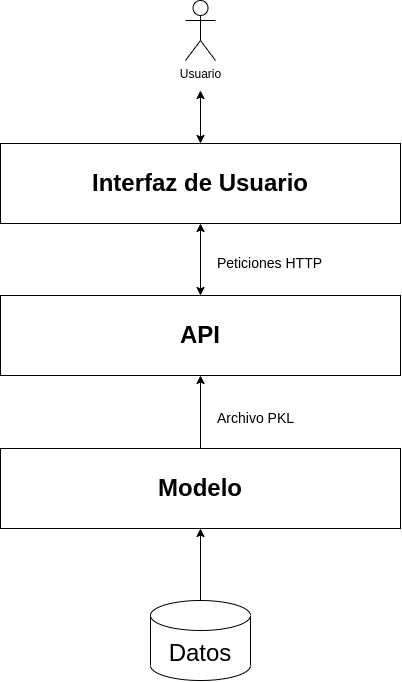
\includegraphics[width=0.50\textwidth]{images/arquitectura-proyecto-de-grado.png}
	\caption{Arquitectura del Sistema}
	\label{fig:arq}
\end{figure}

	La API sirve de middleware o capa intermedia entre el modelo y la interfaz del usuario, es decir, esta se encargaría de recibir los datos de la aplicación web, procesarlos haciendo uso del modelo y devolver el resultado de nuevo a la interfaz para que el usuario pueda verlos.

	Finalmente, la interfaz tiene como finalidad permitir introducir al usuario al sistema, recibir su entrada como una lista de transacciones que están representadas por una fecha y un identificador de cliente, enviar esa información a la API para ser procesada, recibir el resultado y mostrarle un gráfico de probabilidad por cada cliente donde se exprese la probabilidad de que este haya desertado en un punto en el tiempo futuro.
	
	La comunicación entre el modulo del modelo y la API se realizaría mediante un archivo PKL que contiene los parámetros del modelo creado, el cual será importado por la API al momento de su ejecución y utilizado para generar predicciones. La API y la aplicación web hablarían mediante peticiones HTTP e intercambiarían la información en formato JSON.

\section{Requerimientos}

A pesar de que la metodología de desarrollo es ágil, se consideró importante definir una serie de requerimientos como base que debe cumplir el sistema, esto con la finalidad de mantener un enfoque durante la implementación y que las tareas del backlog tengan un objetivo en común.

	Acorde a lo descrito en la sección anterior en la cual se desarrolló una arquitectura para el sistema, la lista de requerimientos por módulo que se estableció es la siguiente: 

\subsection{Modelo}

\subsubsection{Requerimientos Funcionales}

\begin{itemize}
	\item El sistema genera un modelo estadístico que pueda predecir la deserción de clientes de un e-commerce.
\end{itemize}

\subsubsection{Requerimientos no Funcionales}

\begin{itemize}
	\item Se debe importar las transacciones de un archivo CSV.
	\item Se debe procesar la data en un dataframe con las características definidas por la biblioteca lifetimes.
	\item El modelo se debe guardar en un archivo con formato PKL en la carpeta del módulo API.
	\item El código fuente del modelo debe estar disponible dentro del repositorio del proyecto en GitHub.
	\item Se debe implementar el modelo en un Jupyter Notebook.
	\item En el Jupyter Notebook debe estar expresado el proceso de generación del modelo.
	\item Se deben mostrar ejemplos de uso del modelo.
\end{itemize}

\subsection{API}

\subsubsection{Requerimientos Funcionales}

\begin{itemize}
	\item Crear una ruta (/conditional-probability-alive) donde se reciba una lista de transacciones por usuario y se retorne la probabilidad de vida de cada cliente en 500 unidades de tiempo desde la primera transacción.
\end{itemize}

\subsubsection{Requerimientos no Funcionales}

\begin{itemize}
	\item La API será usada por una aplicación web.
	\item La API usará la arquitectura REST.
	\item El formato de entrada y salida debe estar descrito en el archivo README.md correspondiente a la carpeta del proyecto.
	\item Las instrucciones de ejecución deben estar contempladas en el archivo README.md correspondiente a la carpeta del proyecto.
	\item El formato debe especificar en cada campo con su clave y tipo de dato aceptado.
	\item Permitir el acceso libre a la API.
	\item La API debe procesar y retornar datos en formato JSON.
	\item La API debe estar disponible de manera pública mediante un enlace de prueba.
	\item El código fuente de la API debe estar disponible dentro del repositorio del proyecto en GitHub.
\end{itemize}

\subsection{Aplicación Web}

\subsubsection{Requerimientos Funcionales}

\begin{itemize}
	\item El usuario ingresa la lista de transacciones de los clientes y obtiene la probabilidad de que los clientes desertara de su negocio en un grafico lineal.
\end{itemize}

\subsubsection{Requerimientos no Funcionales}

\begin{itemize}
	\item Se debe validar que las fechas ingresadas por el usuario sigan el formato DD-MM-AAAA.
	\item No se pueden ingresar o enviar transacciones sin fecha o identificador de cliente.
	\item El identificador de cliente es una cadena de caracteres con tamaño mayor de tres.
	\item Las instrucciones de ejecución deben estar contempladas en el archivo README.md correspondiente a la carpeta del proyecto.
	\item Se debe describir brevemente las instrucciones de uso en el archivo README.md correspondiente a la carpeta del proyecto.
	\item La aplicación web debe procesar y retornar datos en formato JSON.
	\item Se debe describir brevemente las instrucciones de uso la interfaz.
	\item Se debe acceder a la API mediante un método POST.
	\item El código fuente de la aplicación web debe estar disponible dentro del repositorio del proyecto en GitHub.
\end{itemize}

\section{Diseño de Interfaz de Usuario}

Lo más importante en el sistema es permitir a un usuario ingresar una lista de transacciones de clientes y que este luego pueda ver la probabilidad de que estos clientes deserten, es por ello que se plantea una interfaz simple de una sola página web (ver Figura 2).

\begin{figure}[H]
	\centering 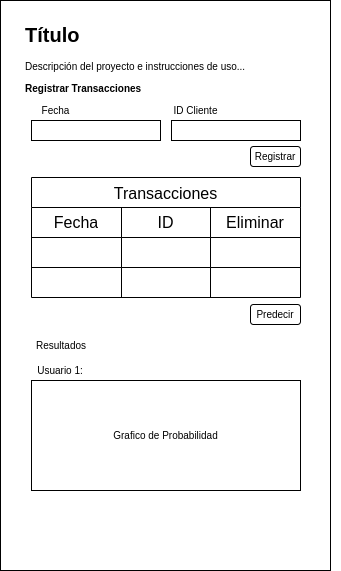
\includegraphics[width=0.50\textwidth]{images/ui.png}
	\caption{Intefaz de Usuario}
	\label{fig:ui}
\end{figure}

La página web inicialmente muestra información sobre el proyecto como título, descripción e instrucciones sobre como utilizar el sistema, luego se muestra un formulario de entrada donde el usuario puede registrar una transacción. La transacción consiste de una fecha en formato DD-MM-AAAA y un identificador de cliente. 

La experiencia de usuario en el sistema es simple, cuando se registra una transacción valida, esta se agrega a una tabla que el usuario puede visualizar con la opción de eliminar alguna transacción ya registrada.

El usuario al terminar de registrar las transacciones hace clic en el botón “predecir”, luego de esto se muestra un gráfico que representa la probabilidad de desertar de un cliente a lo largo del tiempo y comenzando desde la fecha de la primera transacción registrada del cliente. Se construye un grafico por cada identificador de cliente ingresado.
%% Los capitulos inician con \chapter{T'itulo}, estos aparecen numerados y
%% se incluyen en el 'indice general.
%%
%% Recuerda que aqu'i ya puedes escribir acentos como: 'a, 'e, 'i, etc.
%% La letra n con tilde es: 'n.

\chapter{Marco Referencial}

En éste capítulo, se pretende explicar las bases teóricas necesarias para la comprensión del diseño e implementación de un sistema para inferir la deserción de clientes en un e-commerce.

\section{E-Commerce}

Se puede definir al comercio electrónico o E-Commerce como transacciones comerciales realizadas digitalmente entre individuos y organizaciones. Las transacciones comerciales implican un intercambio de valor (por lo general dinero) o comercio entre las partes interesadas a cambio de productos o servicios. El hecho de que se realicen las transacciones digitalmente supone el uso de tecnologías digitales como la internet, la web, dispositivos electrónicos y software.

\subsubsection{Cliente}

Un cliente en el contexto del comercio electrónico es un individuo que realiza compras regulares a través de algún canal digital de una organización. El proceso de compra de este cliente es similar al de una tienda física y consiste en: visualizar los productos o servicios que ofrece la organización, luego procede a agregar lo que desea comprar a un carrito de compras, cuando el cliente está listo para pagar, el carrito es verificado y luego pagado de forma digital, finalmente se genera un registro de pedido en el sistema el cual es procesado por la organización para satisfacer la compra.

\subsubsection{Pedido}

Un pedido u orden de compra es un registro que contiene información relevante sobre una transacción de compra realizada por un cliente en una plataforma de comercio electrónico de una organización. Este registro suele contener información relevante a los procesos de cada organización pero los datos indispensables que incluye son: la fecha en que se realizó un pedido, el valor monetario del mismo y el cliente que lo generó.

\subsubsection{Negocio Contractual}

Se considera negocio contractual a toda organización que interactué y trabaje con sus clientes bajo el modelo de suscripción u otra configuración contractual. En este tipo de organizaciones es relativamente fácil determinar si un cliente está activo o no, ya que por lo general se registran los datos de vencimiento y renovación de contratos o suscripciones. Algunos ejemplos de negocios contractuales son las compañías de seguros, empresas de telecomunicaciones, gimnasios y plataformas SaaS.

\subsubsection{Negocio No Contractual}

Un negocio no contractual es cuando la organización no tiene mecanismo que le ayude a determinar cuando la relación con un individuo o cliente ha finalizado, esto debido a que un cliente puede estar en un periodo de espera antes de realizar otra compra o puede que no compre de nuevo a la organización. Ejemplos de este tipo de negocio son las tiendas de comercio electrónico y las tiendas de venta al por menor.

\subsubsection{Deserción de Clientes (Churn)}

Deserción de clientes o Churn es la pérdida de clientes debido al desgaste y es lo opuesto a la retención de clientes. Ésta se considera una métrica crucial para las empresas y se utiliza como base para calcular otras métricas de gran importancia como la vida útil del cliente, el valor de vida útil (CLV por sus siglas en inglés), el gasto de adquisición de clientes y el gasto de éxito del cliente.

\subsubsection{Valor de vida útil de un cliente (CLV)}

Esta medida representa el valor que tiene un cliente para un negocio a lo largo de toda la relación, es decir, es el valor total que ha aportado un cliente al negocio desde que realizó una primera compra, hasta que desertó.

\section{Modelo}

En líneas generales, un modelo es una representación de un sistema, éste se compone por conceptos que ayudan a explicar el sistema, estudiar los efectos de diferentes componentes y hacer predicciones sobre el comportamiento del mismo. Estos conceptos suelen manifestarse en un grupo de ecuaciones matemáticas.

\subsection{Modelo Estadístico}

Un modelo estadístico es un modelo matemático que representa una o varias suposiciones estadísticas, estas suposiciones tienen describen propiedades que nos permiten calcular la probabilidad de que ocurra un evento.

\subsection{Modelos Buy-Till-You-Die (BTYD)}

Son una familia de modelos estadísticos que tienen como objetivo describir el comportamiento de compra de los clientes como una serie de distribuciones. Estos modelos se basan en dos suposiciones básicas:

\begin{enumerate}
	\item Los clientes interactúan con la organización cuando están activos o "vivos".
	\item Los clientes pueden “morir” o transformarse en clientes inactivos después de un periodo de tiempo.
\end{enumerate}

Existen varios modelos BTYD, pero todos tienen las siguientes características:

\subsubsection{Modelado Probabilístico}

Todos estos modelos generan distribuciones de probabilidad para describir el comportamiento de los clientes. Si bien los modelos difieren en cómo crean estas distribuciones o cómo se ven estas distribuciones, todos comparten este objetivo principal.

\subsubsection{Tabla de pedidos}

La entrada requerida para generar las predicciones en todos los modelos BTYD es simplemente una tabla que contenga los pedidos de los clientes.  Cada modelo procesa esta tabla de manera diferente, pero todos comparten una estructura de entrada común. Debido a este requisito de entrada, cuantos más datos longitudinales se tenga sobre los pedidos de los clientes, más sólidas serán las predicciones del modelo.

\subsubsection{Análisis RFM}

 El modelado y análisis de RFM es una estrategia común empleada actualmente por las empresas para capturar el comportamiento del cliente y clasificarlo según tres variables: 
 
\begin{itemize}
	\item \textbf{Recencia (Recency):} ¿Hace cuánto tiempo compró un cliente? Este dato hace referencia a la duración en periodos de tiempo entre la primera compra del cliente y la última.	
	\item \textbf{Frecuencia (Frecuency):} ¿Con qué frecuencia/consistencia compra un cliente? Este valor representa la cantidad de periodos de tiempo en los que el cliente realizó un pedido.
	\item \textbf{Valor Monetario (Monetary):} ¿Cuánto gasta un cliente en promedio? Esto es la suma de todos los valores monetarios de las compras de un cliente dividida por el número total de compras.
\end{itemize}

Cada uno de estos elementos del análisis RFM juega un papel clave en las distribuciones del los modelos BTYD. 

\subsection{Modelo Pareto / NBD}

El nombre se refiere a la distribución de Pareto utilizada para modelar la deserción de clientes y la distribución binomial negativa (NBD) utilizada en la predicción de compras futuras. Este modelos asume que los clientes compran a un ritmo constante durante un periodo de tiempo y luego pasan a la inactividad.

	El objetivo del modelo Pareto / NBD es desarrollar el análisis RFM capturando el contexto del cliente al decidir si, el cliente ha desertado o no y con qué frecuencia comprará. Por ejemplo, si estudiamos un cliente A y un cliente B: 

\begin{itemize}
	\item El cliente A compró en una tienda de comercio electrónico cada dos días durante 2 meses. Sin embargo, no ha comprado en las últimas 2 semanas.
	\item El cliente B compró en la tienda aproximadamente una vez al mes durante los últimos 6 meses. Tampoco ha comprado en las últimas 2 semanas.
\end{itemize}

A pesar de que ambos clientes tienen la misma antigüedad (14 días), la diferencia en el comportamiento de compra cambia la probabilidad de deserción. Además, a pesar de comprar en la misma tienda, exhiben patrones de compra significativamente diferentes (cada dos días frente a cada mes), por lo que cualquier predicción debe tener en cuenta sus hábitos de compra.

El modelo de Pareto/NBD se basa en cinco supuestos:

Desde el punto de vista del cliente individual:

\begin{itemize}
	\item \textbf{Compras siguen la distribución Poisson:} Mientras está activo, el número de transacciones realizadas por un cliente en un período de tiempo de longitud t se representan mediante una distribución Poisson con media $\lambda t$. En realidad, Pareto/NBD, como su nombre lo indica, utiliza una distribución binomial negativa de la cual, la distribución de Poisson es un caso especial. La distribución de Poisson es una elección acertada para modelar el tiempo entre transacciones, ya que diferentes negocios tendrán diferentes tiempos y los clientes también pueden exhibir diferentes patrones de compra.
	\item \textbf{“Vida útil” exponencial:} Cada cliente tiene una "vida útil" no observada de longitud $\tau$. Este punto en el que el cliente se vuelve inactivo se distribuye exponencialmente con una tasa de deserción $\mu$. Esto lo que nos dice es que en general, la mayoría de los clientes se transformarán en inactivos relativamente rápido después de realizar una compra inicial pero una pequeña cohorte de clientes permanecerá durante mucho tiempo.
\end{itemize}

Heterogeneidad entre clientes:

\begin{itemize}
	\item \textbf{Las tasas de compra individuales siguen la distribución gamma:} la tasa de compra $\lambda$ para los diferentes clientes sigue una distribución gamma entre la población de clientes.
	\item \textbf{Tasa de deserción sigue distribuciones gamma diferentes:} Las tasas de deserción $\mu$ siguen una distribución gamma que es diferente entre los clientes.
	\item \textbf{Independencia de tasas:} Las tasas de transacciones $\lambda$ y las tasas de deserciones $\mu$ están distribuidas independientemente entre ellas.
\end{itemize}

Este modelo tiene mucho poder a la hora de analizar el comportamiento de clientes y requiere solo dos entradas sobre cada cliente, su "recencia" y "frecuencia". El modelo utiliza la inferencia de probabilidad logarítmica para hacer predicciones sobre el futuro. Un problema de este modelo es que su implementación puede ser desafiante desde el punto de vista computacional debido al uso prolongado de la función hipergeométrica gaussiana.

\subsection{Modelo BG / NBD}

Este modelo deriva del modelo Pareto / NBD como una alternativa simple de calcular desde el punto de vista computacional. Su nombre hace referencia a la distribución geométrica beta utilizada para modelar la deserción de clientes y la distribución binomial negativa (NBD) utilizada en la predicción de compras futuras. 

	La mayoría de los aspectos del modelo BG / NBD reflejan directamente los del modelo Pareto / NBD. La única diferencia radica en las consideraciones que definen cómo y cuándo los clientes se vuelven inactivos. La distribución de tiempo de Pareto asume que la deserción puede ocurrir en cualquier momento, independientemente de la ocurrencia de compras reales, en este modelo se asume que el abandono ocurre inmediatamente después de una compra, permitiendo así modelar este proceso mediante la distribución geométrica beta (BG por sus siglas en inglés).

El modelo de BG / NBD se basa en cinco supuestos :

\begin{enumerate}
	\item Mientras está activo, el número de transacciones realizadas por un cliente representan mediante una distribución Poisson con una tasa de transacciones $\lambda$. Esto es equivalente a suponer que el tiempo entre transacciones se distribuye exponencialmente con tasa de transacción $\lambda$.
	\item La tasa de compra $\lambda$ para los diferentes clientes sigue una distribución gamma entre la población de clientes.
	\item Después de cualquier transacción, un cliente se vuelve inactivo con probabilidad p. Por lo tanto, el punto en el que el cliente "abandona" se distribuye entre las transacciones de acuerdo con una distribución geométrica (desplazada).	
	\item Las tasas de transacciones $\lambda$ y las tasas de deserciones $\mu$ están distribuidas independientemente entre ellas.
	\item La heterogeneidad en p sigue una distribución beta.
\end{enumerate}

El modelo BG / NBD se puede implementar de una manera relativamente sencilla y eficiente, además de que la estimación de sus parámetros no requiere ningún software especializado ni la evaluación de funciones matemáticas no convencionales.

\section{Data}

Datos o data en inglés, es una representación simbólica de un atributo o variable cuantitativa o cualitativa. Los datos describen hechos empíricos, sucesos y entidades, es decir, transmiten información. 

Los datos son indispensables en la investigación científica, las finanzas y en prácticamente cualquier otra forma de actividad organizacional humana. Ejemplos de conjuntos de datos incluyen precios de acciones, tasas de delincuencia, pedidos de clientes en un e-commerce, tasas de desempleo, tasas de alfabetización y datos del censo.
	
\subsection{Dataset}

Un Dataset se puede definir como un conjunto de información en particular, representado en una tabla o matriz de análisis. La tabla está conformada por columnas y cada una de ellas representa una variable de datas, las filas suponen un grupo de datos específicos.

\section{Herramientas Tecnológicas}

Datos o data en inglés, es una representación simbólica de un atributo o variable cuantitativa o cualitativa. Los datos describen hechos empíricos, sucesos y entidades, es decir, transmiten información. 

Los datos son indispensables en la investigación científica, las finanzas y en prácticamente cualquier otra forma de actividad organizacional humana. Ejemplos de conjuntos de datos incluyen precios de acciones, tasas de delincuencia, pedidos de clientes en un e-commerce, tasas de desempleo, tasas de alfabetización y datos del censo.
	
\subsection{Python}

Python es un lenguaje de programación dinámico de propósito general extremadamente popular. Éste lenguaje soporta múltiples paradigmas de programación como lo son la programación orientada a objetos, la programación funcional y la programación estructurada. Su filosofía hace énfasis en la legibilidad del código mediante el uso de indentación y se considera una de las herramientas principales en área de las ciencias de datos.
	
\subsection{Biblioteca Lifetimes}

Lifetimes es una biblioteca de software que implementa los modelos estadísticos Buy-Till-You-Die, Customer Lifetime Value y el modelo bayesiano PyMC (en Beta) en el lenguaje de programación Python. Es de código abierto bajo la licencia Apache 2.0.
	
\subsection{Biblioteca Pandas}

Pandas es una biblioteca de software escrita para el lenguaje de programación Python, comúnmente usada para la manipulación y el análisis de datos. Ofrece estructuras de datos y operaciones para manipular datos de forma tabular y series de tiempo. Es software libre publicado bajo la licencia BSD de tres cláusulas.
	
\subsection{Biblioteca MatplotLib}

Matplotlib es una biblioteca de gráficos para el lenguaje de programación Python. Se utiliza para incrustar gráficos en aplicaciones y poder visualizar los datos o resultados de modelos. Es de código abierto y se distribuye bajo la licencia de estilo BSD.
	
\subsection{Jupyter Notebook}

Jupyter Notebook (anteriormente IPython Notebook) es un entorno computacional interactivo muy popular en la ciencia de datos, el cual se ejecuta en la web y se utiliza para crear documentos que simulan un cuaderno digital. Cada documento contiene una lista ordenada de celdas de entrada/salida que pueden contener código de programación, texto (usando el formato Markdown), lenguaje matemático, diagramas e imágenes. 
	
\subsection{Flask}

Flask es un framework de Python que se utiliza para crear aplicaciones y sistemas web. Este framework no requiere otro tipo de herramientas y bibliotecas, tampoco tiene componentes preexistentes lo que lo hace muy ligero. Es de código abierto bajo la licencia BSD y fue lanzado inicialmente en abril del año 2010.

\subsection{Javascript}

Javascript es un lenguaje de programación dinámico de alto nivel, es interpretado y su sintaxis se basa en los lenguajes C++ y Java. Todos los navegadores web modernos interpretan el código Javascript por lo que se considera el lenguaje de la web, se utiliza principalmente para añadir dinamismo a las páginas web en el lado del cliente, pero actualmente se utiliza también en el lado del servidor para crear aplicaciones de todo tipo.

\subsection{Typescript}

Typescript es un lenguaje de programación tipado, compilado y de código abierto bajo la licencia Apache. Fue desarrollado en Octubre del año 2012 y actualmente es mantenido por Microsoft como un subconjunto del lenguaje de programación Javascript.  

El uso y popularidad de Typescript ha crecido exponencialmente en los últimos años debido a las mejoras que ofrece sobre el lenguaje Javascript, en especial la validación de tipos para las variables lo cual ayuda en la detección temprana de errores aumentando la robustez del software, se considera esencial para proyectos grandes.

\subsection{Vue.js}

Vue.js es un framework de código abierto escrito en Typescript que se utiliza en la construcción de interfaces de usuario dinámicas y aplicaciones web. Fue creado por Evan You en febrero del año 2014 bajo la licencia MIT. Este framework es de los más populares actualmente para crear interfaces web y se enfoca en una arquitectura de representación declarativa y composición de componentes. 

\subsection{Nuxt}

Nuxt es un metaframework que utiliza como base a Vue.js, es de código abierto bajo la licencia MIT y tiene como objetivo facilitar la creación de aplicaciones web “universales”, es decir, sitios web que tengan la funcionalidad de una aplicación web y los beneficios de los sitios web estáticos. Fue creado en octubre del 2016 por Sebastien Chopin, Alexandre Chopin y Pooya Parsa.

\subsection{Chart.js}

Es una biblioteca gratuita de código abierto para la visualización de datos, está escrita en Javascript y fue creada en el año 2013 bajo la licencia MIT. Esta biblioteca permite mostrar datos en gráficos de barra, linea, área, circular, burbujas, radar, polar y de dispersión, todo esto utilizando la tecnología de HTML5 Canvas. Es una de las bibliotecas mas populares y se considera la mejor por su simplicidad de uso.

%% Los capitulos inician con \chapter{T'itulo}, estos aparecen numerados y
%% se incluyen en el 'indice general.
%%
%% Recuerda que aqu'i ya puedes escribir acentos como: 'a, 'e, 'i, etc.
%% La letra n con tilde es: 'n.

\chapter{Conclusiones y Recomendaciones}

En este proyecto se logró definir, diseñar e implementar un sistema con el fin de predecir la deserción de clientes de una tienda de comercio electrónico, para esto se ejecutó una metodología de desarrollo ágil que consistía en un conjunto de requerimientos, los cuales tenían como finalidad cumplir los objetivos propuestos para el proyecto y que luego fueron desglosados en un backlog de tareas, para finalmente ser implementadas mediante un tablero Kanban.

	Todo comenzó con una investigación para definir el modelo correcto que posibilitara predecir la deserción de clientes dado un listado de transacciones, concluyendo así en un modelo de la familia “Buy Till You Die” llamado BG / NBD, luego se examinó la web para obtener un dataset que permitiese ajustar los parámetros  del modelo seleccionado.

	Al tener el modelo se definió una arquitectura del sistema, se implementó cada uno de los módulos y se desplegó en varios servidores para que pueda ser usado. En base a los resultados obtenidos se puede observar que, efectivamente el sistema logra predecir la deserción de clientes en un ambiente continuo y de carácter no contractual como lo es una tienda de comercio electrónico.

	El sistema desarrollado en este proyecto puede servir fácilmente como base para futuros proyectos enfocados en mejorar la experiencia de los clientes en ambientes no contractuales, y así  identificar oportunidades de re-conversión, de ventas de valor agregado y optimizar los objetivos de negocios de las empresas que trabajen en el ámbito del e-commerce.
	
	Como recomendaciones encontradas durante el desarrollo de este sistema, hemos planteado las siguientes:

\begin{itemize}
	\item Para obtener mejores resultados, sería ideal que la data utilizada para la construcción del modelo sea el historial de transacciones real de la tienda de comercio electrónico que lo usaría, esto debido a que el comportamiento de los clientes suele variar según la categoría de productos que se venden, la región o país del mundo, el tipo de clientes y otros factores que puedan influir en las decisiones de compra.
	\item Tomando en cuenta lo anterior, se recomienda integrar el sistema como una extensión o herramienta en plataformas de comercio electrónico populares como Magento, WooCommerce, Vendure, Shopify, etc.
	\item Si se usaran los datos de compra y clientes de una tienda de comercio electrónico activa, sería necesario actualizar el modelo de vez en cuando, como sugerencia se puede  construir el modelo anualmente.
	\item Para el despliegue del sistema se recomienda utilizar un servicio de despliegue de código automatizado como Heroku, Digital Ocean Apps, Railway o configurar un servidor que haga uso del sistema operativo Linux.

\end{itemize}

%% Los capitulos inician con \chapter{T'itulo}, estos aparecen numerados y
%% se incluyen en el 'indice general.
%%
%% Recuerda que aqu'i ya puedes escribir acentos como: 'a, 'e, 'i, etc.
%% La letra n con tilde es: 'n.

\chapter{Conclusiones y Recomendaciones}

En este proyecto se logró definir, diseñar e implementar un sistema con el fin de predecir la deserción de clientes de una tienda de comercio electrónico, para esto se ejecutó una metodología de desarrollo ágil que consistía en un conjunto de requerimientos, los cuales tenían como finalidad cumplir los objetivos propuestos para el proyecto y que luego fueron desglosados en un backlog de tareas, para finalmente ser implementadas mediante un tablero Kanban.

	Todo comenzó con una investigación para definir el modelo correcto que posibilitara predecir la deserción de clientes dado un listado de transacciones, concluyendo así en un modelo de la familia “Buy Till You Die” llamado BG / NBD. Luego se examinó la web para obtener un dataset que permitiese ajustar los parámetros  del modelo seleccionado.

	Al tener el modelo se definió una arquitectura del sistema, se implementó cada uno de los módulos y se desplegó en varios servidores para que pueda ser usado. En base a los resultados obtenidos se puede observar que, efectivamente el sistema logra predecir la deserción de clientes en un ambiente continuo y de carácter no contractual como lo es una tienda de comercio electrónico.

	El sistema desarrollado en este proyecto puede servir fácilmente como base para futuros proyectos enfocados en mejorar la experiencia de los clientes en ambientes no contractuales, y así  identificar oportunidades de re-conversión, de ventas de valor agregado y optimizar los objetivos de negocios de las empresas que trabajen en el ámbito del e-commerce.
	
	Como recomendaciones encontradas durante el desarrollo de este sistema, hemos planteado las siguientes:

\begin{itemize}
	\item Para obtener mejores resultados, sería ideal que la data utilizada para la construcción del modelo sea el historial de transacciones real de la tienda de comercio electrónico que lo usaría, esto debido a que el comportamiento de los clientes suele variar según la categoría de productos que se venden, la región o país del mundo, el tipo de clientes y otros factores que puedan influir en las decisiones de compra.
	\item Tomando en cuenta lo anterior, se recomienda integrar el sistema como una extensión o herramienta en plataformas de comercio electrónico populares como Magento, WooCommerce, Vendure, Shopify, etc.
	\item Si se usaran los datos de compra y clientes de una tienda de comercio electrónico activa, sería necesario actualizar el modelo de vez en cuando, como sugerencia se puede  construir el modelo anualmente.
	\item Para el despliegue del sistema se recomienda utilizar un servicio de despliegue de código automatizado como Heroku, Digital Ocean Apps, Railway o configurar un servidor que haga uso del sistema operativo Linux.

\end{itemize}


\appendix
%% Cap'itulos incluidos despues del comando \appendix aparecen como ap'endices
%% de la tesis.
%\include{apendiceA}
%\include{apendiceB}
%\include{apendiceC}

%% Incluir la bibliograf'ia. Mirar el archivo "biblio.bib" para m'as detales
%% y un ejemplo.

\bibliographystyle{apalike}
\bibliography{biblio}

\end{document}
